
%% Refer to latex document when possible
\pdfoutput=1
\documentclass[10pt]{beamer}

%STANDARD PREAMBLE
%https://tex.stackexchange.com/questions/68821/is-it-possible-to-create-a-latex-preamble-header
\usepackage{/Users/mwojno01/Research/LabMeetings/beamer_preamble}




\title{The Multivariate Normal Model}
%\subtitle{}

\begin{document}

\maketitle

\begin{frame}{Table of contents}
  \setbeamertemplate{section in toc}[sections numbered] \tableofcontents[hideallsubsections]
\end{frame}


\section{Overview}
\subsection{Motivations}
\begin{frame}{Some motivations for the normal}

\begin{figure}
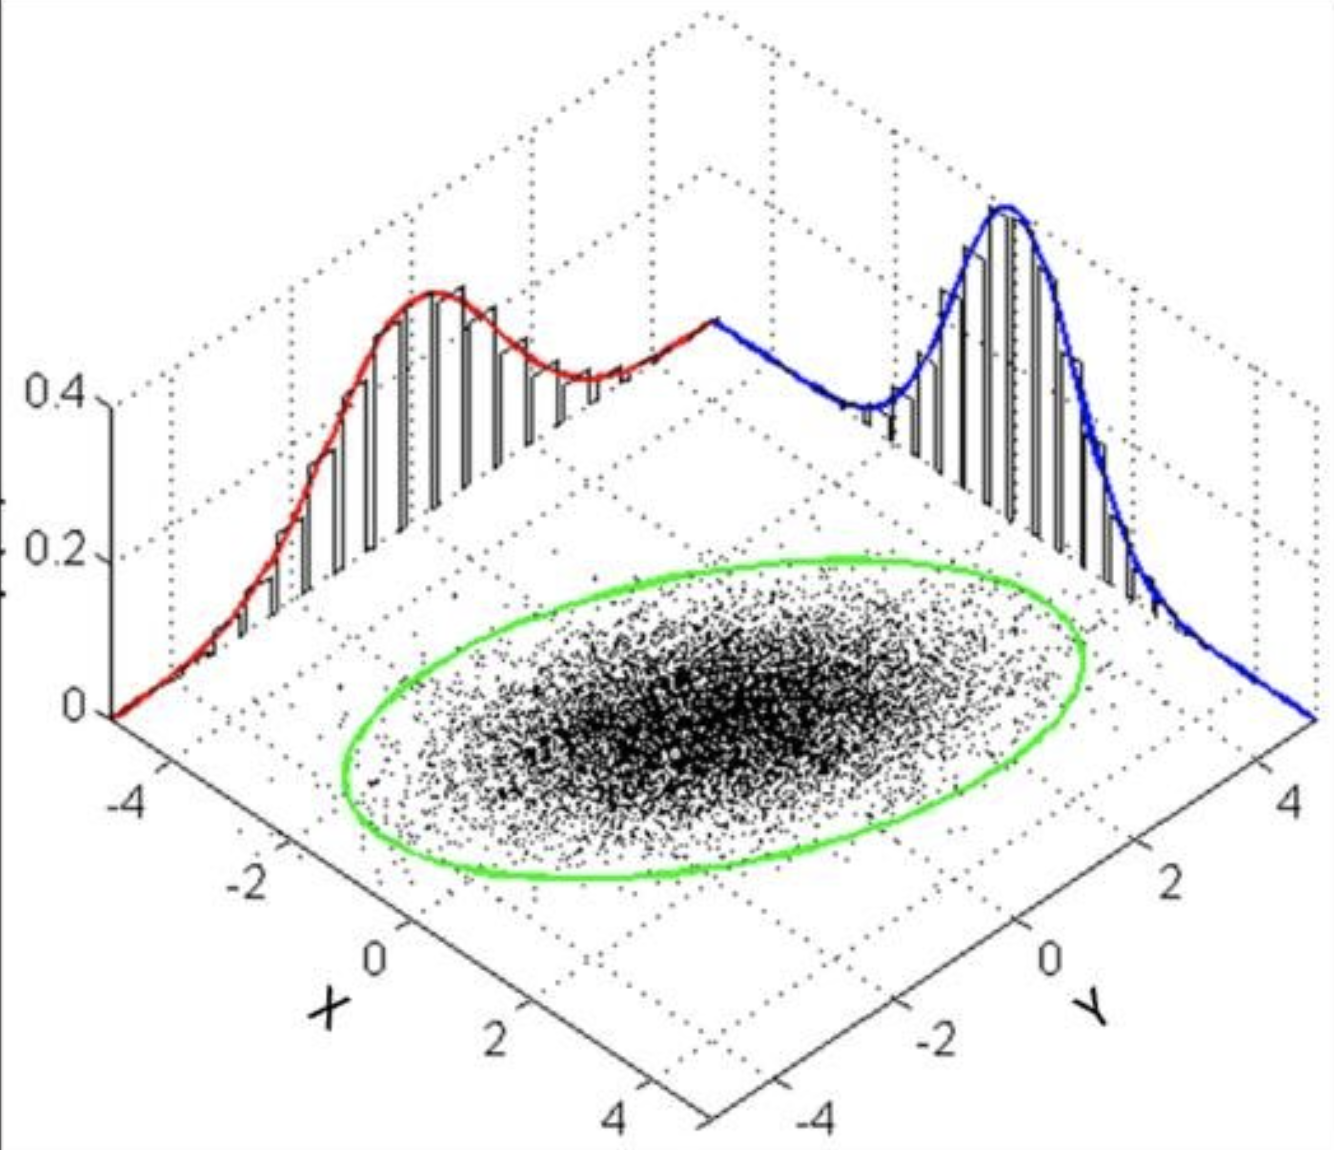
\includegraphics[width=.3\textwidth]{images/mvn}
\end{figure}

\begin{itemize}
	\item \textit{Maximum entropy} among all distributions with a given mean $\+\mu$ and variance $\+\Sigma$.  \pause
	\item Characterized by independence of sample mean and sample variance. {\footnotesize (Bayesian take: ask if your beliefs about the sample mean are independent from those about the sample variance.)} \pause
	\item Sample averages are generally approximately normally distributed due to the Central Limit Theorem. \pause 
	\item Sufficient statistics are sample mean and variance; so will consistently estimate population mean and variance even for non-normal distributions.
\end{itemize}
\end{frame}


\begin{frame}{Why \alert{Bayesian} normal? }
\begin{itemize}
\item Prior information often exists and can be taken into account.
	\begin{itemize}
	\item Population-level info {\tiny (Previous example: disease prevalence.  Forthcoming example: biometrics and PIMA Indians)}
	\item Nature (e.g. support) of data {\tiny (Forthcoming example: reading comprehension)}
	\end{itemize} \pause 	
\item ML estimates of covariance matrices can have large variance.
	\begin{itemize}  
	\item Problem can be especially bad in certain contexts {\tiny ( e.g., small data, high-dimensions, missing data)}
	\item Spherical prior provides regularization
	\item Posterior still asymptotically concentrates around maximum likelihood (ML) solution
	\end{itemize} \pause 
\item Inference can be as easy or easier than in frequentist models
	\begin{itemize}
	\item Easy, cheap updates {\scriptsize (esp. when using a conjugate prior)}
	\item Supports online learning 	
	\item Fits nicely in more complex models	
	%\item Nice hyperparameter interpretation
	\end{itemize}
\end{itemize}	
\end{frame}

\subsection{Building blocks}
\begin{frame}{Review: Exponential families}

We have observed that the Bernoulli and the Poisson distributions are both \blue{\href{https://github.com/mikewojnowicz/exponential_family/blob/297dde8bf81b09544b66f3b80324db44bc601358/exponential_family.pdf}{exponential families.}}
 
\metroset{block=fill}
\begin{block}{Exponential family}
An \textit{exponential family} is a set of probability distributions whose probability density functions have the following form
\begin{align*}
\labelit \label{eqn:exponential_family}
 p(x \cond \theta) = h(x) \exp \{ \eta(\theta)^T t(x) - a(\theta)\} 
\end{align*}
where we refer to $h$ as the base measure, $\eta$ as the natural parameter, $t$ as the sufficient statistics, and $a$ as the log normalizer. 
\end{block}
\end{frame}

\begin{frame}{Multivariate normal is an exponential family} 
We can write the density of a \blue{\href{https://en.wikipedia.org/wiki/Multivariate_normal_distribution}{multivariate normal}} $\N(\+\mu, \+\Sigma)$ distribution in exponential form. \textit{(Try it!)}\pause 
\scriptsize
\begin{align*}
& p(\+x \cond \+\mu, \+\Sigma) = (2\pi)^{-d/2} |\+\Sigma |^{-1/2} \exp \bigg\{ -\half (\+x - \+\mu)^T \+\Sigma^{-1} (\+x - \+\mu) \bigg\}  \\
& = (2\pi)^{-d/2} \exp \bigg\{ -\half \explaintermbrace{$\redmathbox{-\half \vectorize (\+\Sigma^{-1})}^T \greenmathbox{\vectorize (\+x\+x^T)} $}{\+x^T \+\Sigma^{-1} \+x} + \redmathbox{(\Sigma^{-1} \+\mu)}^T \greenmathbox{\+x} \bluemathbox{-\half \+\mu^T \+\Sigma^{-1} \+\mu + \half \log |\+\Sigma^{-1} |} \bigg\} 
\labelit \label{eqn:mvn_as_ef} 
\intertext{\tiny \hfill Note: the underbrace representation is given by $\+x^T \+\Sigma^{-1} \+x = \tr (\+x^T \+\Sigma^{-1} \+x) = \tr (\+\Sigma^{-1} \+x \+x^T) =\vectorize (\+\Sigma^{-1})^T \vectorize (\+x\+x^T)$. } 
\end{align*} 
%\footnote{Recall $\tr(\+A\+B) = \vectorize (\+A)^T \vectorize (\+B)$.}  
\pause 
\begin{itemize}
\item \textbf{Natural parameter}: $\eta(\+\mu, \+\Sigma) = \redmathbox{\big(-\half \vectorize (\+\Sigma^{-1}) , \,  \+\Sigma^{-1} \+\mu \big)} $, \item \textbf{Sufficient statistics}: $t(\+x) = \greenmathbox{\big(\vectorize (\+x \+x^T), \+x \big)}$, 
\item \textbf{Log normalizer}: $a(\+\mu, \+\Sigma) =  \bluemathbox{-\half \+\mu \+\Sigma^{-1} \+\mu + \half \log |\+\Sigma^{-1} |} $. 
\item \textbf{Base measure}: $h(x) = (2\pi)^{-d/2}$ 
\end{itemize}
\end{frame}

\begin{frame}{Qualitative points}
	
\metroset{block=fill}
\begin{block}{The natural parametrization of the MVN}
From Equation \eqref{eqn:mvn_as_ef}, we see that that the natural parameters of the MVN are 
\begin{itemize}
\item  the \textit{precision} $\+\Sigma^{-1}$ , and 
\item the \textit{precision-weighted mean} $\+\Sigma^{-1} \+\mu$. 
\end{itemize}
\end{block}

\vfill 

\metroset{block=fill}
\begin{block}{Are you exponentiating a quadratic?}
We also see that if a random vector $\+x$ has a density on $\R^d$ that satisfies
 \[ p(\+x) \propto \exp \{ -\half \+x^T \+A \+x + \+x^T \+b\} \] 
 for some matrix $\+A$ and vector $\+b$, then $\+x$ must be multivariate normal. Moreover its natural parameters are precision $\+A$ and precison-weighted mean $\+b$.  In other words, the covariance is $\+A^{-1}$ and the mean is $\+A^{-1}\+b$. 
\end{block}
\end{frame}

\begin{frame}{Self-help guide for deriving Gibbs samplers}
\begin{center}
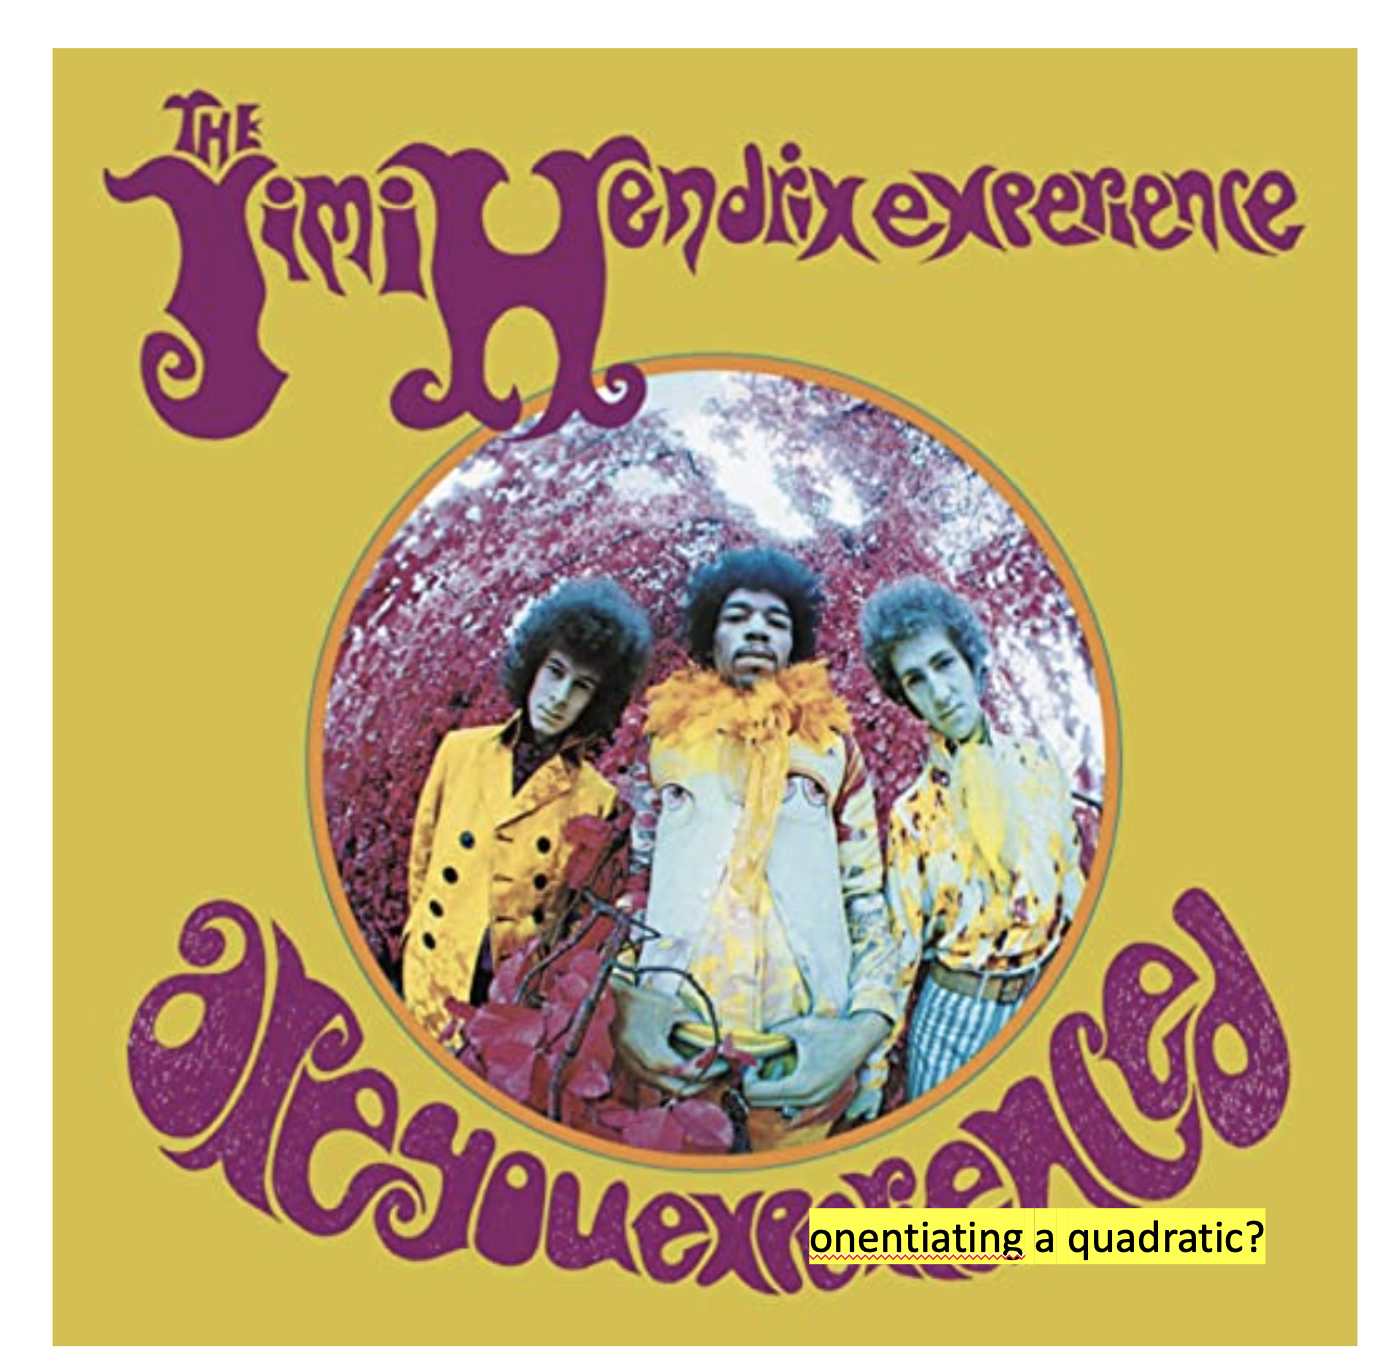
\includegraphics[width=.8\textwidth]{images/are_you_exponentiating_a_quadratic}	
\end{center}

\end{frame}

\begin{frame}{Inverse Wishart Distribution}
The Inverse Wishart is a distribution on symmetric,  positive definite matrices.     The Inverse Wishart distribution,  denoted $\InverseWishart(\nu, \+\Psi)$,  has density

\begin{align}
p(\+\Sigma) \propto | \+\Sigma|^{-(\nu+d +1) /2}  \exp \bb{ -\df{1}{2} \tr ( \+\Sigma^{-1} \+\Psi) } 
\label{eqn:inverse_wishart_density}
\end{align}
where $\+\Sigma \succ 0$ and $\nu > d-1$ to have a proper prior.     The expected value of an Inverse Wishart random variable parametrized as in \eqref{eqn:inverse_wishart_density} is given by $\E[\+\Sigma] = \frac{\+\Psi}{\nu -d -1}$.   

\metroset{block=fill}
\begin{block}{Interpreting the parameters of the Inverse Wishart}
Note that the parameters of the Inverse Wishart can be interpreted {\tiny (as per conjugacy; we will see this below) } in the following way: the covariance was estimated from $\nu$ observations with a residual sum of squares (a.k.a.  sum of pairwise deviation products) $\+\Psi$. 
 \end{block}

\end{frame}

\begin{frame}{Inverse Wishart Distribution}

\vfill 
\begin{center}
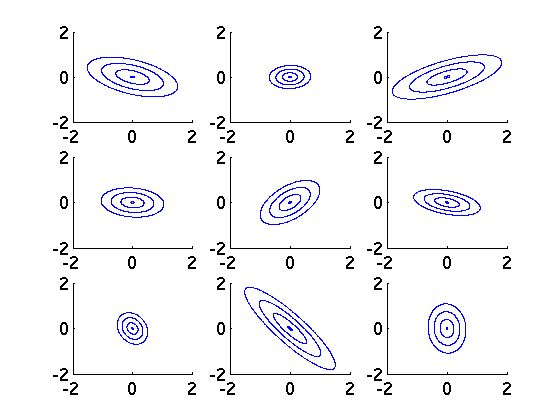
\includegraphics[width=.7\textwidth]{images/inverse_wishart_samples}
\end{center}
\vfill 
\bottomtext{\hfill Image Credit: Michael Hughes, Tufts University}

\end{frame}

\begin{frame}{Sampling from the Inverse Wishart}
A sample $\+\Sigma$ from the $\InverseWishart(\nu, \+\Psi)$ distribution  can be obtained by the following scheme:

\begin{enumerate}
\item Sample $\+z_1, ..., \+z_{\nu} \iid \N (\+0,  \+\Psi^{-1})$
\item Calculate $\+Z^T \+Z = \sum_{i=1}^\nu \+z_i \+z_i^T$.
\item Set $\+\Sigma = ( \+Z^T \+Z )^{-1}$.
\end{enumerate}
The intuition is that the Inverse Wishart models covariance matrices as an inverse sum of squares.
\end{frame}

%%%%%%%%%%%%%%%		
\section{Conjugate inference}



\begin{frame}{A fully conjugate formulation}

Since the MVN is an EF, we can form a fully conjugate model.

\metroset{block=fill}
\begin{block}{Fully conjugate Bayesian MVN {\tiny (has \alert{closed-form} posteriors and predictive posteriors!)} }
Given observations $\+x := (\+x_1,  \hdots \+x_N)$,  where each $\+x_i \in \R^d$, we take

\metroset{block=fill}
\begin{align*}
\+\mu, \+\Sigma &\sim \NIW_d(\alpha_0, \+\mu_0, \nu_0, \+\Psi_0 )  \\
\+x_i \cond \+\mu,  \+\Sigma &\iid \N_{d}( \+\mu , \+\Sigma), \quad i=1,...,N
\end{align*}
\end{block}

\pause 
\begin{block}{The Normal-Inverse-Wishart prior}
	\begin{align*}
\+\mu, \+\Sigma &\sim \NIW_d(\alpha_0, \+\mu_0, \nu_0, \+\Psi_0 ) 
\intertext{which means}
\+\Sigma &\sim \InverseWishart_d(\nu_0,  \+\Psi_0) \\
\+\mu \cond \+\Sigma &\sim \N_d(\+\mu_0, \frac{1}{\alpha_0} \Sigma )
\end{align*}
\end{block}

\end{frame}

\begin{frame}{Application: Modeling typing dynamics}

See powerpoint slides.	
\end{frame}

%%%%%
\section{Semi-conjugate inference}

\begin{frame}{Semi-conjugate Bayesian normal}

\metroset{block=fill}
\begin{block}{Semi-conjugate Bayesian MVN}
Consider the following model with a normal sampling distribution and \textit{semi-conjugate} prior 
\begin{align*}
\+\mu &\sim \N_{d}(\+m_0,\+V_0 ) \\
\+\Sigma &\sim \InverseWishart(\nu_0,  \+\Psi_0) \\
\+x_i \cond \+\mu,  \+\Sigma &\iid \N_{d}( \+\mu , \+\Sigma), \quad i=1,...,N
\end{align*}
We define $\+x := (\+x_1,  \hdots \+x_N)$,  where each $\+x_i \in \R^d$.
\end{block}



 %The conditionally conjugate prior lacks closed-form posterior updating,  but is also more expressive.    It is also easier to extend upwards.

\end{frame}

\begin{frame}{Semi-conjugate models: Gist}
\alert{Main idea:}  A family of prior distributions for a parameter is called \textit{semi-conjugate} if the conditional posterior distribution (often called the \textit{complete conditional}),  given the data and all other parameters in the model,  is also in that family.
\vfill

\metroset{block=fill}
\begin{block}{Comparison}
\begin{columns}
    \begin{column}{.45\linewidth}
	Fully conjugate model 
	\begin{itemize}
	\item $(\+\mu, \+\Sigma) \cond \text{rest}$ is Normal-Inverse-Wishart
	\end{itemize}
	\end{column}
    \begin{column}{.45\linewidth}
	    Semi-conjugate model
	\begin{itemize}
	\item $\+\mu \cond \text{rest}$ is Normal
	\item $\+\Sigma \cond \text{rest}$ is Inverse Wishart	
	\end{itemize}
    \end{column}
\end{columns}
\end{block}

\vfill
\pause 
\metroset{block=fill}
\begin{block}{Relative evaluation of semi-conjugate model} \pause 
\begin{itemize}
\item[] \redx lacks closed-form posterior updating \pause 
\item[] \greencheck more expressive \pause 
\item[] \greencheck easier to embed in more complex models 
\end{itemize}
\end{block}
	
\end{frame}

\begin{frame}{Semi-conjugate models: Definition}

\begin{sblock}{Review: Conjugate models}
Conjugacy was defined as follows \cite{gelman2013bayesian}. If $\mathcal{F}$ is a class of sampling distributions and $\mathcal{P}$ is a class of prior distributions for $\theta$, then the class $\mathcal{P}$ is \textit{conjugate} for $\mathcal{F}$ if
\[  p(\redmathbox{\theta} \cond \bluemathbox{y} ) \in \mathcal{P} \; \text{for all} \; p(\cdot \cond \redmathbox{\theta}) \in \mathcal{F} \; \text{and} \; p(\cdot) \in \mathcal{P} \]
\end{sblock}

\begin{sblock}{Semi-conjugate models}
Semi-conjugate (sometimes called conditionally-conjugate) models can be defined similarly  \cite{gelman2013bayesian}.  If $\mathcal{F}$ is a class of sampling distributions and $\mathcal{P}$ is a class of prior distributions for $\theta \cond \phi$, then the class $\mathcal{P}$ is \textit{conditionally conjugate} for $\mathcal{F}$ if
\[  p(\redmathbox{\theta} \cond \greenmathbox{\phi}, \bluemathbox{y}) \in \mathcal{P} \; \text{for all} \; p(\cdot \cond \redmathbox{\theta}, \greenmathbox{\phi}) \in \mathcal{F} \; \text{and} \; p(\cdot \cond \greenmathbox{\phi}) \in \mathcal{P} \]
\end{sblock}
\end{frame}


{
\usebackgroundtemplate{%
\tikz\node[opacity=0.3] {
\includegraphics[height=\paperheight,width=\paperwidth]{images/hearts_and_cupid}};}
	\begin{frame}{We {\red \heart} semi-conjugacy}	 
	 In general, semi-conjugate models do not have closed-form posteriors.  
	 \vfill 
	 Why are they of interest?  \pause 
	 \vfill 
	 The posterior distributions are easily approximated 
	 \begin{itemize}
	 \item with \textbf{Gibbs sampling}, by sampling from the complete conditionals
	 \item with \textbf{mean-field variational inference}, by taking variational expectations of the natural parameters of the complete conditional.	
	 \end{itemize}  
	 
	\end{frame}
}

\begin{frame}{The complete conditional for $\+\mu$}

\scriptsize We use the exponential family representation of the MVN  to represent the prior in terms of its natural parameters
\begin{align*}
	p(\+\mu) &\propto \exp \bigg\{ -\half \+\mu^T \bigg( \explaintermbrace{prior precision}{\+V_0^{-1}} \bigg) \+\mu + \+\mu^T \bigg(\explaintermbrace{prior precision-weighted mean}{\+V_0^{-1} \+m_0}  \bigg) \bigg\} 
\labelit \label{eqn:prior_for_mvn_fixed_cov}
\end{align*}

And similarly, we write the likelihood $	L(\+\mu) = p(\+y \cond \+\mu) = \prod_{i=1}^n p(\+y_i \cond \+\mu)$  as
\begin{align*}
	L(\+\mu) &\propto \exp \bigg\{ -\half \ds\sum_{i=1}^n (\+x_i - \+\mu)^T \+\Sigma^{-1} (\+x_i - \+\mu)\bigg\}  \\
	&= \exp \bigg\{ - \half \+\mu^T \bigg(\explaintermbrace{data precision}{n \+\Sigma^{-1}}\bigg) \+\mu + \+\mu^T \bigg(\explaintermbrace{data precision-weighted mean}{\+\Sigma^{-1} n \bar{\+x}} \bigg) \bigg\} 
\labelit \label{eqn:likelihood_for_mvn_fixed_cov}
\end{align*}


\textit{Can you finish the derivation? (Hint: Remember Jimi!)} \pause  
By Bayes' law, and combining like terms,
\begin{align*}
 p(\+\mu \cond \+x, \+\Sigma) &\propto \explaintermbrace{prior}{p(\+\mu)}\explaintermbrace{likelihood}{p(\+x \cond \+\mu, \+\Sigma)} \\
 &= \exp \bigg\{ - \half \+\mu^T \bigg( \explaintermbrace{posterior precision}{\+V_0^{-1} + n  \+\Sigma^{-1}}\bigg)  \+\mu + \+\mu^T \bigg( \explaintermbrace{posterior precision-weighted mean}{\+V_0 \+m_0 + \+\Sigma^{-1} n \bar{\+x}} \bigg) \bigg\} 
\end{align*}
which reveals that the posterior is normal,  along with the particular form of its parameters  %(covariance $\+A^{-1}$ and mean $\+A^{-1} \+b$). 

\end{frame}

	

\begin{frame}{Complete conditionals for the Bayesian MVN}
The complete conditions under natural parametrization
\footnotesize 
\begin{align*}
\+\mu  \cond \+\Sigma, \+x &\sim \N_{d}(\+m,\+V ) \\ %\labelit\label{eqn:normal_model_complete_conditional_on_mu} \\
\intertext{where}
\explaintermbrace{posterior precision}{\+V^{-1}} &= \explaintermbrace{prior precision}{\+V_0^{-1}} +  \explaintermbrace{data precision}{n \+\Sigma^{-1}}  \\
\explaintermbrace{posterior precision-weighted mean}{\+V^{-1} \+m}  &=  \explaintermbrace{prior precision-weighted mean}{\+V_0^{-1} \+m_0} + \explaintermbrace{data precision-weighted mean}{n \+\Sigma^{-1}  \bar{\+x}}  
\intertext{and}
\+\Sigma \cond \+\mu,  \+x  &\sim \InverseWishart(\nu,  \+\Psi) \\
%\labelit \label{eqn:normal_model_complete_conditional_on_Sigma} \\
\intertext{where}
\explaintermbrace{posterior sample size}{\nu} &=  \explaintermbrace{prior sample size}{\nu_0} + \explaintermbrace{sample size}{n} \\
\explaintermbrace{posterior RSS}{\+\Psi} &= \explaintermbrace{prior RSS}{\Psi_0} + \explaintermbrace{data RSS}{\ds\sum_{i=1}^n  (\+x_i - \+\mu) (\+x_i - \+\mu)^T}
%\labelit \label{eqn:Sigma_cc_normal_model_cond_conj_prior}\\ 
\end{align*}
\bottomtext{\hfill Note: RSS = Residual Sum of Squares}
\end{frame}

\begin{frame}{Gibbs Sampler {\scriptsize (in standard parametrization)}}
	
We sample from the posterior by iteratively sampling from the \textit{complete conditionals}:
\footnotesize 
\begin{align*}
\+\mu  \cond \+\Sigma, \+x &\sim \N_{d}(\+m,\+V ) \\ %\labelit\label{eqn:normal_model_complete_conditional_on_mu} \\
\intertext{where}
\+V &= \bp{\explaintermbrace{prior precision}{\+V_0^{-1}} +  \explaintermbrace{data precision}{n \+\Sigma^{-1}} }^{-1} \\
\+m  &=  \+V  \bp{\explaintermbrace{prior precision-weighted mean}{\+V_0^{-1} \+m_0} + \explaintermbrace{data precision-weighted mean}{n \+\Sigma^{-1}  \bar{\+x}} } 
\intertext{and}
\+\Sigma \cond \+\mu,  \+x  &\sim \InverseWishart(\nu,  \+\Psi) \\
%\labelit \label{eqn:normal_model_complete_conditional_on_Sigma} \\
\intertext{where}
\nu &=  \nu_0 + n \\
\+\Psi &= \Psi_0 + \ds\sum_{i=1}^N  (\+x_i - \+\mu) (\+x_i - \+\mu)^T 
%\labelit \label{eqn:Sigma_cc_normal_model_cond_conj_prior}\\ 
\end{align*}
\end{frame}


 
\begin{frame}{Complete conditionals: Interpretation}
These complete conditionals have nice interpretations:
\begin{itemize}
\item \textbf{Complete conditional for $(\+\mu  \cond \+\Sigma, \+x)$}: On the precision scale,  $\+V$ is the sum of the prior precision matrix $\+V_0^{-1}$ and the data precision matrix (which is $N$ copies of the precision for each observation,  $\+\Sigma^{-1}$).    Similarly,  $\+m$ is the precision-weighted convex combination of $\+m_0$, the prior mean,    and the empirical average, $\bar{\+x}$.
\item \textbf{Complete conditional for $(\+\Sigma \cond \+\mu,  \+x)$}:  The covariance was estimated from $\nu$ observations with a sum of pairwise deviation products $\Psi$.
\end{itemize}
\end{frame}




	
	

%%%%%
\section{Application: Reading Comprehension}

\begin{frame}

See ipython notebook. 	
\end{frame}


%%%%%
\section{Missing data and imputation}

\begin{frame}{References}

\begin{center}
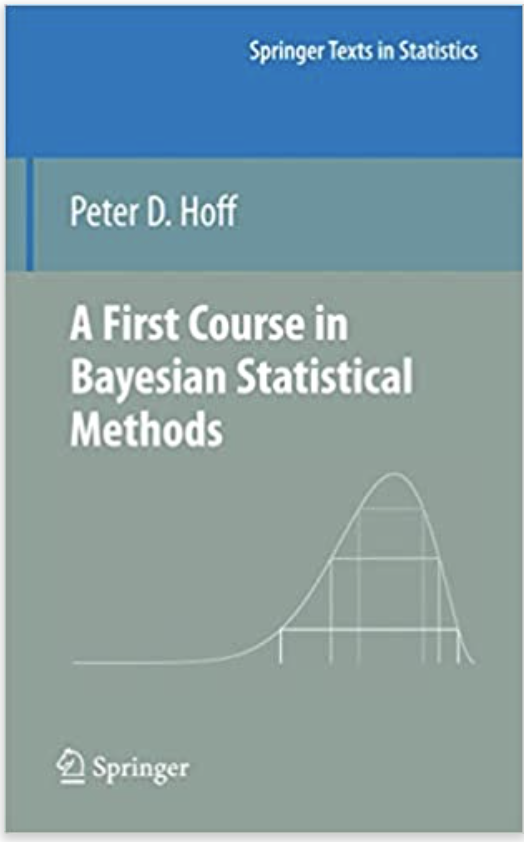
\includegraphics[width=.5\textwidth]{images/hoff_book}
\end{center}

\end{frame}

\begin{frame}{Pima Dataset}

\begin{figure}
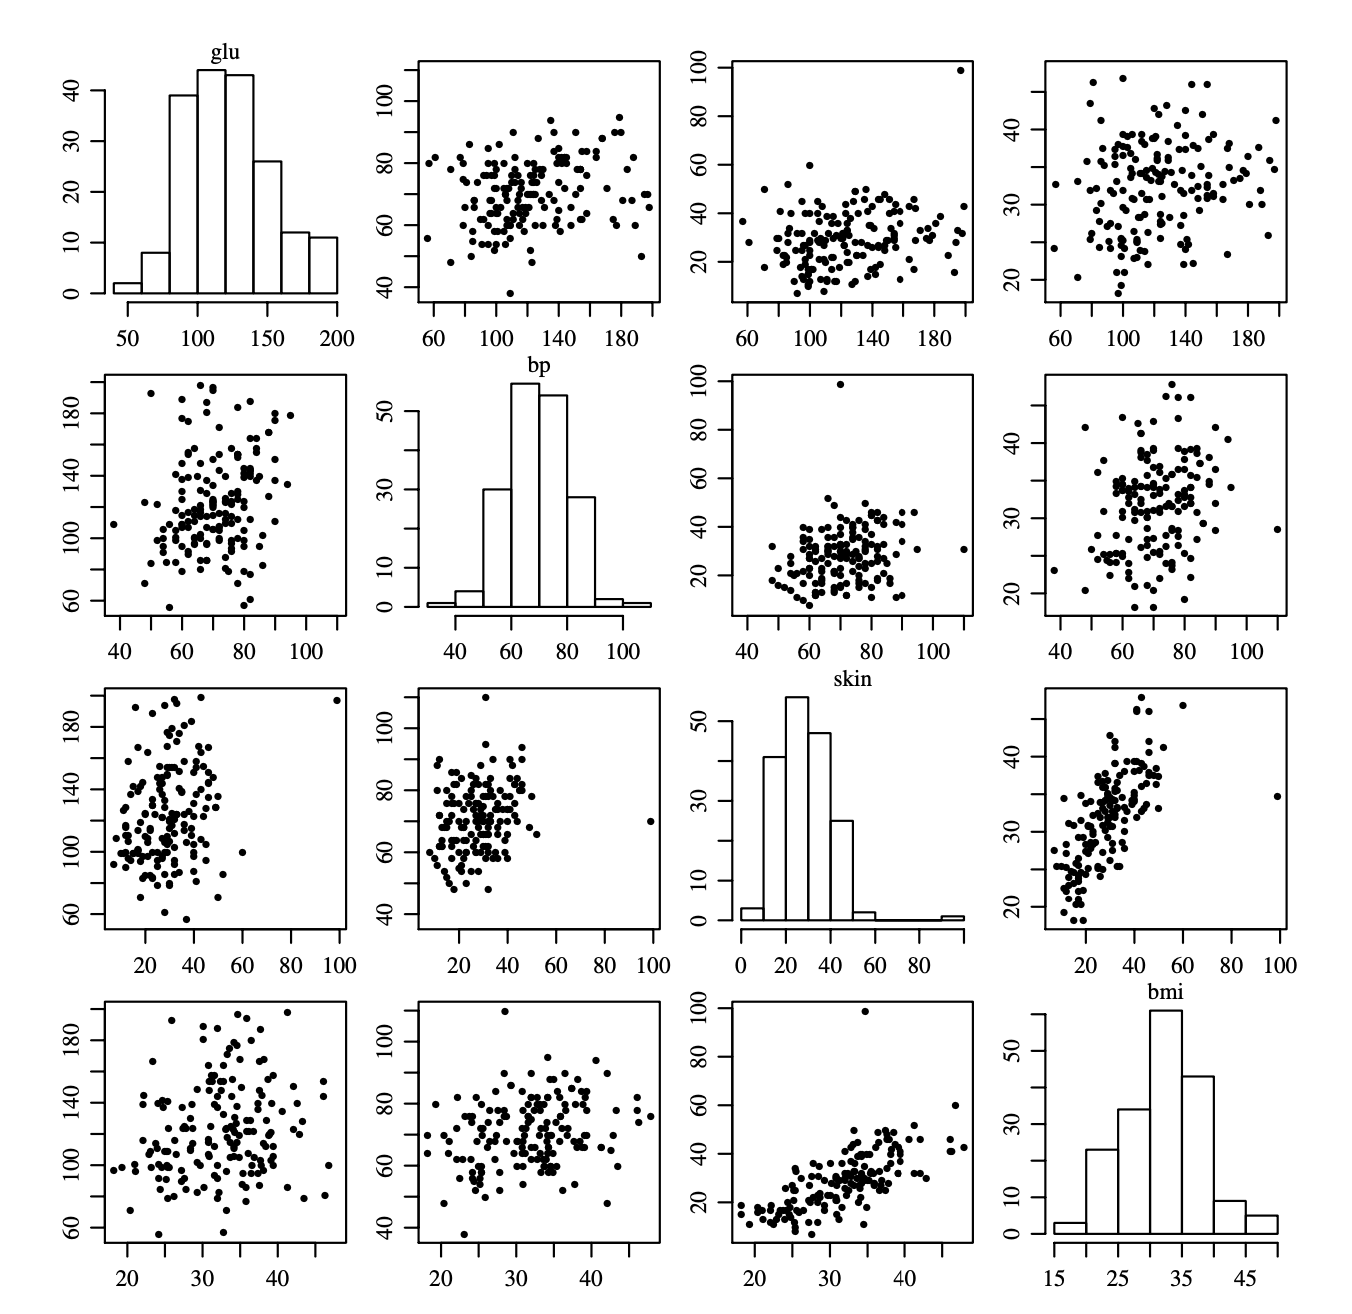
\includegraphics[width=.6\textwidth]{images/pima_scatterplots}
\caption{  \footnotesize Univariate histograms and bivariate scatterplots for four variables taken from a dataset involving health-related measurements on 200 women of Pima Indian heritage living near Phoenix,  Arizona.  \scriptsize The four variables are \texttt{glu} (blood plasma glucose concentration),  \texttt{bp} (diastolic blood pressure),  \texttt{skin} (skin fold thickness),  and  \texttt{bmi} (body mass index).  }
\end{figure}

\end{frame}

\begin{frame}{Pima Dataset}

\begin{figure}
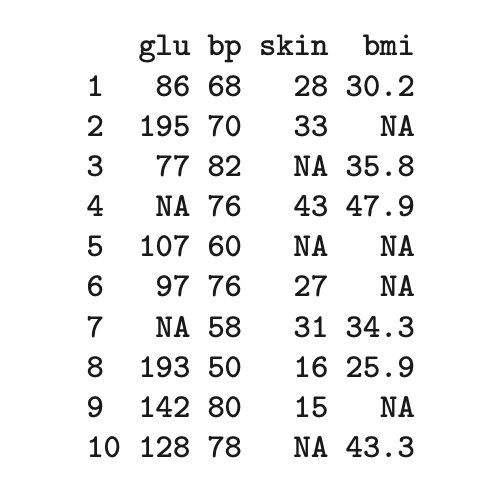
\includegraphics[width=.6\textwidth]{images/pima_first_ten_entries}
\caption{  \footnotesize Entries for the first ten subjects in the dataset.  \scriptsize The \texttt{NA}'s stand for ``not available." }
\end{figure}
\end{frame}

\begin{frame}{Description of problem}
How to do parameter estimation in the presence of missing data? \\
\begin{itemize}
\item[]  \footnotesize  We cannot do parameter estimation,  because we cannot compute the likelihood $\prod_{i=1}^n p(\+y_i \cond \+\theta)$.  \normalsize
\end{itemize}
\vfill \vfill 
Two common approaches taken by software packages:
\begin{enumerate}
\item Throw away all subjects with missing data
\pause  \\
\quad \redx \footnotesize Discards a potentially large amount of useful information.  \normalsize
\pause \\
\item  Impute the population mean or some other fixed value. 
\pause \\
\quad \redx \footnotesize  Assumes certainty about these values,  when in fact we have not observed them.  \normalsize
% DELIVERY: Elicit audience suggestions as to the problems with each common approach.
\end{enumerate}
\end{frame}


\begin{frame}{Missing at random (MAR)}
Let $\+O_i = (O_1, ..., O_p)^T$ be a binary vector such that
\begin{itemize}
\item $O_{ij} = 1 \implies  Y_{ij}  \; \text{is observed}$ 
\item $O_{ij} = 0 \implies  Y_{ij}  \; \text{is missing}$ 
\end{itemize}

\vfill

\begin{definition}
We say the missing data are \textit{missing at random} if $\+O_i$ and $\+Y_i$ are conditionally independent given the model parameters  $\+\theta$  and the distribution of $\+O_i$ does not depend on $\+\theta$.
% TODO: Check this definition;  I altered Hoff's to be more clear based on what seemed to be used in the upcoming formula.
\end{definition}


\vfill  \vfill \vfill  \pause 

\scriptsize
\textbf{Remark.}  This is one of the three types of missingness.   In gist:
\begin{itemize}
\item Missing completely at random (MCAR) - missingness is independent of all data
\item Missing at random (MAR) - missingness is independent of observed data
\item Missing not at random (MNAR) - missingness depends on missing values (and perhaps observed data)
\end{itemize}
% QUESTION: Does this characterization (grabbed from some slides) comport with the one I gave for MAR above? No mention of parameters here.   Perhaps the frequentist characterization differs form the Bayesian one?


\end{frame}


\begin{frame}{The likelihood in the presence of MAR data}

When the data is missing at random,  the sampling probability (density) for the data from observational unit $i$ is given by

\begin{align*}
p(\+o_i,  \set{y_{ij} : o_{ij} =1} \cond \+\theta) & \stackrel{(1)}{=} p(\+o_i) \;  p(\set{y_{ij} : o_{ij} =1} \cond \+\theta) \\
&=  p(\+o_i) \;  \ds\int p(y_{i1}, ...., y_{ip}  \cond \+\theta)  \prod_{y_{ij} : o_{ij} = 0} dy_{ij}
\end{align*}
\footnotesize where in (1) we applied the definition of MAR. \normalsize

\vfill \vfill \pause

\greencheck So in the presence of MAR data, the correct thing to do is \textit{integrate over} the missing data to obtain the marginal probability (density) of the observed data. 
\end{frame}


\begin{frame}{Utilization in multivariate normal models}


In the case of multivariate normal models \footnotesize (so $\+\theta = (\+\mu, \+\Sigma)$) \normalsize, the integration is easy:  Multivariate normals have normal marginals. 

\vfill \vfill \vfill 
\begin{example}
Suppose $\+y_i = (y_{i1},  \texttt{NA},  y_{i3},  \texttt{NA})^T$, so $\+o_i = (1,0,1,0)^T$.     

Then

\begin{align*}
p(\+o_i,  y_{i1},  y_{i3} \cond \+\mu, \+\Sigma) & = p(\+o_i) \;  p(y_{i1},  y_{i3} \cond \+\mu, \+\Sigma) \\
&=  p(\+o_i) \;  \ds\int p( \+y_i  \cond \+\mu, \+\Sigma)  \; dy_2 \; dy_4
\end{align*}
\vfill 

The marginal density $p(y_{i1},  y_{i3} \cond \+\theta)$ is simply a bivariate normal density with mean $(\mu_1,  \mu_3)^T$ and covariance matrix made up of $(\sigma^2_1,  \sigma_{13},  \sigma^2_3)$.
\end{example}

\end{frame}

\begin{frame}{Gibbs sampling with missing data}

\begin{sblock}{Complete data}
If $\+Y$ is the $n \times p$ matrix in which $o_{i,j}=1$ if $Y_{i,j}$ is observed and $o_{i,j} = 0$ if $Y_{i,j}$ is missing, then $\+Y$ has two parts

\begin{itemize}
\item $\+Y_{\text{obs}} := \{y_{i,j} : o_{i,j} =1 \}$, the data that we observe, and 
\item 	$\+Y_{\text{miss}} := \{y_{i,j} : o_{i,j} =0 \}$, the data that we do not observe.
\end{itemize}
\end{sblock}

\begin{sblock}{Gibbs sampler}
A Gibbs sampling scheme for approximating the posterior is given by:

\begin{enumerate}
\item Sampling $\+\mu^{(s+1)}$ from $p(\+\mu \cond \+Y_{\text{obs}}, \+Y_{\text{miss}}^{(s)}, \+\Sigma^{(s)})$;
\item Sampling $\+\Sigma^{(s+1)}$ from $p(\+\Sigma \cond \+Y_\text{obs}, \+Y_\text{miss}^{(s)}, \+\mu^{(s+1)})$;
\item Sampling $\+Y_\text{miss}^{(s+1)}$ from $p(\+Y_\text{miss} \cond \+Y_\text{obs}, \+\mu^{(s+1)}, \+\Sigma^{(s+1)})$;
\end{enumerate}
\end{sblock}

\pause
\bottomtext{The first two steps are the same as before!  The third step is covered in the next slide.  Any guesses?}

\end{frame}


\begin{frame}{Sampling the missing data}

\scriptsize 
\begin{align*}
p(\+Y_\text{miss} \cond \+Y_\text{obs}, \+\mu, \+\Sigma) & \propto p(\+Y_\text{miss},  \+Y_\text{obs} \cond  \+\mu, \+\Sigma) \\
&= \ds\prod_{i=1}^n p(\+y_{i, \text{miss}}, \+y_{i, \text{obs}} \cond \+\mu, \+\Sigma) \\
&\propto \ds\prod_{i=1}^n p(\+y_{i, \text{miss}} \cond \+y_{i, \text{obs}},  \+\mu, \+\Sigma) \\
\end{align*}

How to proceed? \pause  We apply standard results about conditional distributions formed from partitions of multivariate normals:

\begin{align*}
\+y_{[b]} \cond \+y_{[a]}, \+\mu, \+\Sigma & \sim \mathcal{MVN} \bigg( \+\mu_{b|a}, \+\Sigma_{b|a}  \bigg), \quad \text{where} \\
\+\mu_{b|a} &= \+\mu_{[b]} + \+\Sigma_{[b,a]} (\+\Sigma_{[a,a]})^{-1} (\+y_{[a]} - \+\mu_{[a]}) \\
\+\Sigma_{b|a}  &= \+\Sigma_{[b,b]} -  \+\Sigma_{[b,a]} (\+\Sigma_{[a,a]})^{-1} 	\Sigma_{[a,b]}
\end{align*}

\bottomtext{Some macroscopic properties:  \pause 
	\begin{itemize}
	\item The conditional mean, $\+\mu_{b|a}$, starts off at the unconditional mean, $\+\mu_{[b]}$, but then is modified by $(\+y_{[a]} - \+\mu_{[a]})$ in a way that depends on the covariance $\+\Sigma_{[b,a]}$.
	\item The conditional variance $\+\Sigma_{b|a}$ is less than the unconditional variance $\+\Sigma_{[b,b]}$  
	\end{itemize}
}

\end{frame}

\begin{frame}{Posterior Correlations}

\begin{columns}
\begin{column}{0.6\textwidth}

To each covariance matrix there corresponds a correlation matrix $\+C$ given by
\[ \+C := \bigg\{c_{jk} : c_{jk} = \Sigma_{[j,k]} / \sqrt{\Sigma_{[j,j]} \Sigma_{[k,k]}} \bigg\} \]

Simply taking the mean across samples, we obtain the approximation
\[ \E[\+C \cond \+y_1, ..., \+y_n] = 
\begin{bmatrix}
1.00 & 0.23 & 0.25& 0.19 \\
0.23& 1.00& 0.25& 0.24 \\	
0.25& 0.25& 1.00& 0.65 \\	
0.19 &0.24&0.65&1.00 \\		
\end{bmatrix}
\]

\scriptsize 
Notes:
\begin{itemize}
\item Bayesian paradigm again yielding unlimited access to posterior functionals of interest,  without doing any extra inferential work!   % Compare to frequentist or variational inference 
\item Correlations are generally of interest for multivariate normal models, but they are \textit{especially} relevant to imputation. % used to improve how misssing values are filled in.
\end{itemize}
\end{column}

\begin{column}{0.4\textwidth}
\begin{figure}
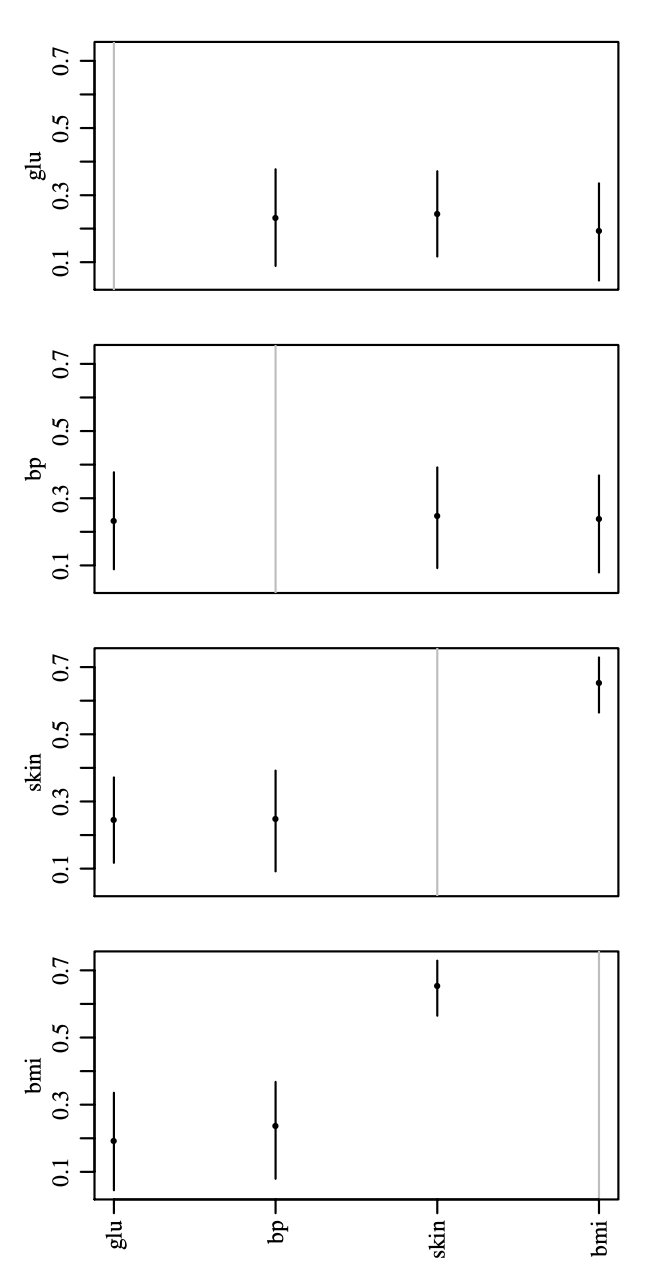
\includegraphics[width=.7\textwidth]{images/pima_correlations}
\caption{95\% posterior confidence intervals for correlations}
\end{figure}
\end{column}


\end{columns}
 \end{frame}

\begin{frame}{Intelligent imputations}
The posterior expectation gives a much better imputation than some flat fixed value.

\begin{figure}
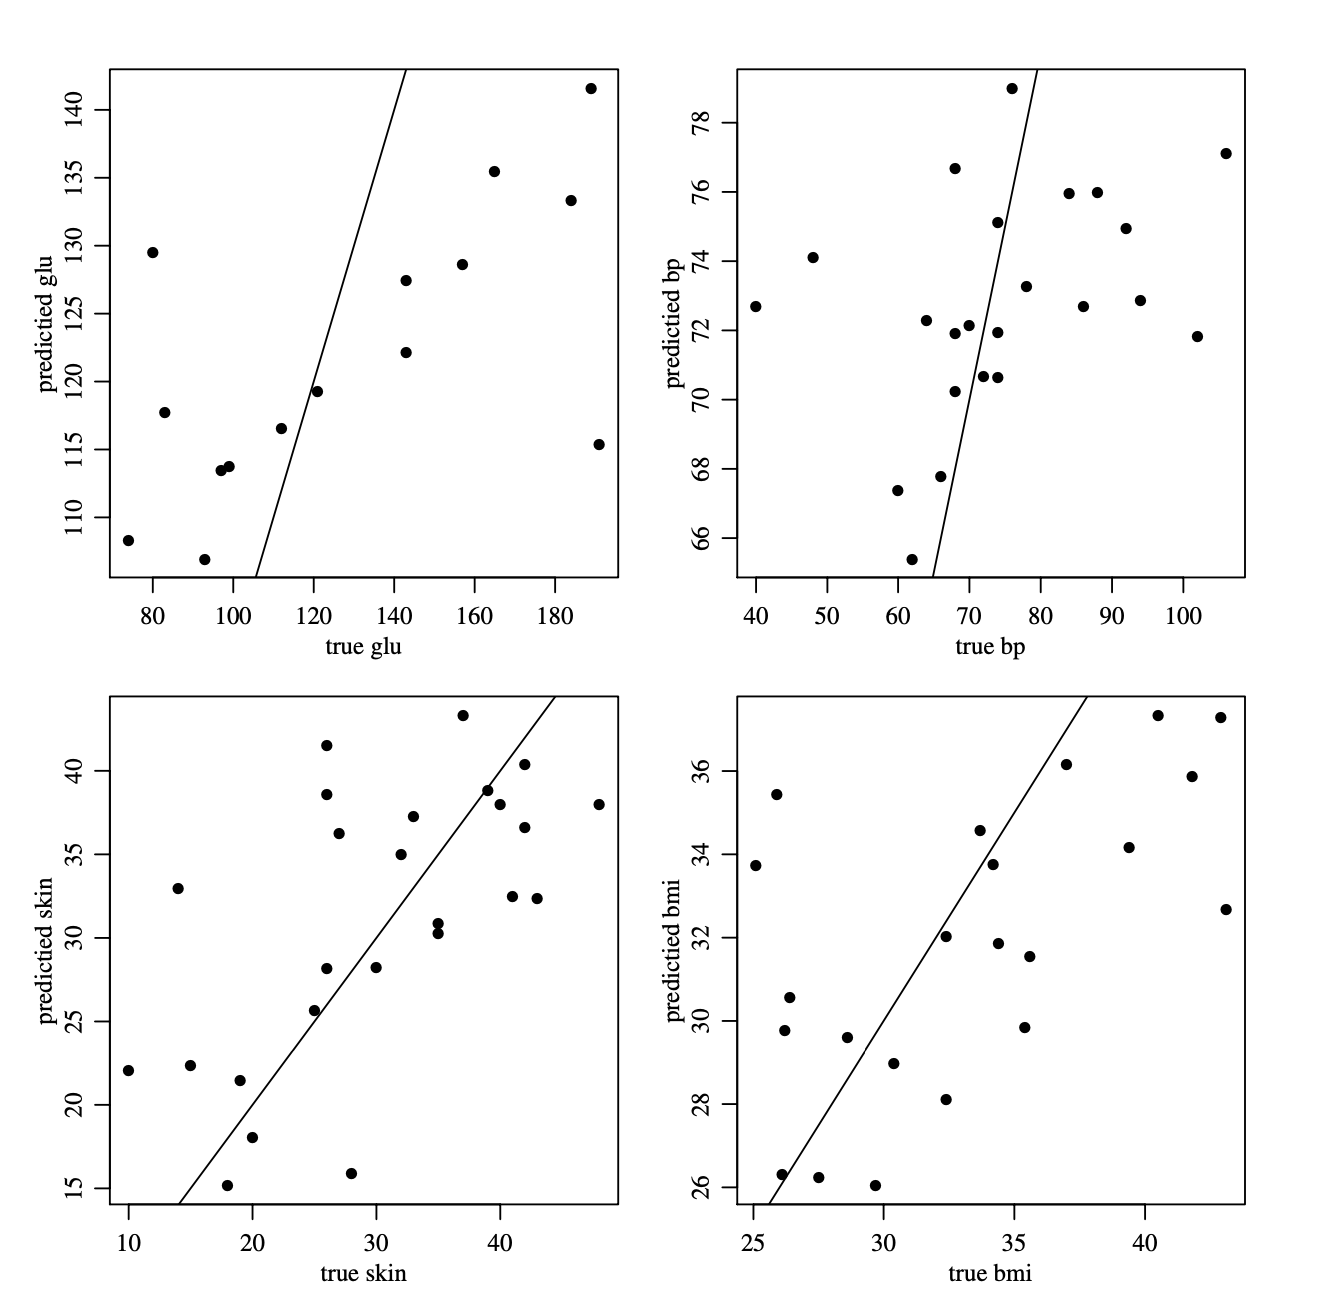
\includegraphics[width=.45\textwidth]{images/pima_missing_vs_true}
\caption{True values of the missing data vs. posterior expectations}
\end{figure}

\pause 
 Imputations are especially good for \texttt{skin} and \texttt{bmi},  due to their higher correlations.  

\end{frame}



\end{document}



